\section{GUI}\label{gui}

Die GUI (Grafic User Interface) wurde nur mit den Android bzw. GooglePlay Services (inkl. Googlemaps) um gesetzt. Die mitgelieferten
M�glichkeiten des Android SDK sind in dieser Hinsicht f�r die GUI-Umsetzung dieses Projektes vollkommen zufriedenstellend. Die komplette
GUI setzt sich aus 2 Activities zu sammen, die im folgenden n�her beleuchtet werden.

\subsection*{Login-Screen}
Diese Activity wird zuerst aufgerufen und zeigt einen Bildschirm auf dem sich der Spieler einen Benutzernamen aussucht und danach mit dem
"`Start"' Button zu n�chsten Activity wechselt, welche das eigentliche Spiel zeigt.

\begin{wrapfigure}{r}{0.5\textwidth}
  \begin{center}
    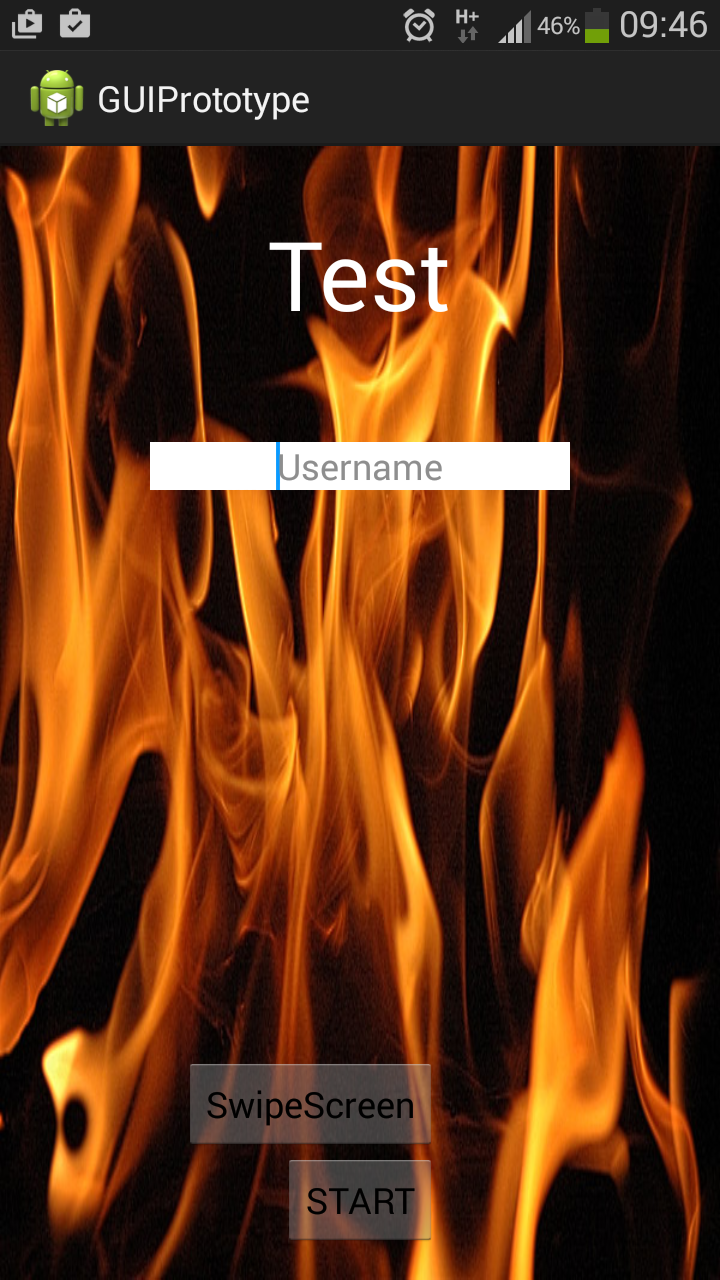
\includegraphics[width=0.48\textwidth]{4-Technische_Loesungen/4-5-GUI/Data/login_screen.png}
     \caption{Login Screen}
  \end{center}
\end{wrapfigure}


\subsection*{Swipe-Screen}
Schon in der sehr fr�hen Entwicklungsphase war festzustellen, das die verschiedenen Elemente der GUI - wie im folgenden weiter erl�utert- zu zahlreich sind, um sie auf einen Bildschirm umzusetzen. Die eigentliche Kartendarstellung w�re sonst zu klein gewesen. Also wurde entschieden die verschiedenen Elemente auf weitere Bildschirme zu verteilen. In den ersten Entw�rfen geschah dies �ber einzelne Activities, also mehrere Bildschirme. Um gewisse Android Komfort-Funktionen und Gesten dem Nutzer zu verf�gung zu stellen wurden die zun�chst eigenst�ndigen Activites zu Fragments umgebeut, die dann in einem so genannten Swipe-Screen zusammengefasst werden. In diesem werden die Fragments als Tabs organisiert und der User kann entweder durch "`wischen"' (swipe) oder durch klicken auf die Tabs durch die GUI Navigieren. \newline
Ein weiterer Vorteil ist ebenfalls, dass benachbarte Tabs jeweils vorgeladen (Laden der Widgets) bzw. noch im Speicher behalten werden. Zum einen wird so sichergestellt, dass der Tab-Wechsel per wischen "`geschmeidig"' abl�uft. Dadurch ergeben sich auch sehr geringe Ladezeiten zwischen den einzelenen Bildschirmen. Zudem ist die von Google angepriesene "`Wiederverwendbarkeit"' von Fragments als UI (User Interface) ebenfalls n�tzlich, wenn weitere �hnliche Spiele umgesetzt werden sollen.

\begin{wrapfigure}{r}{0.5\textwidth}
  \begin{center}
    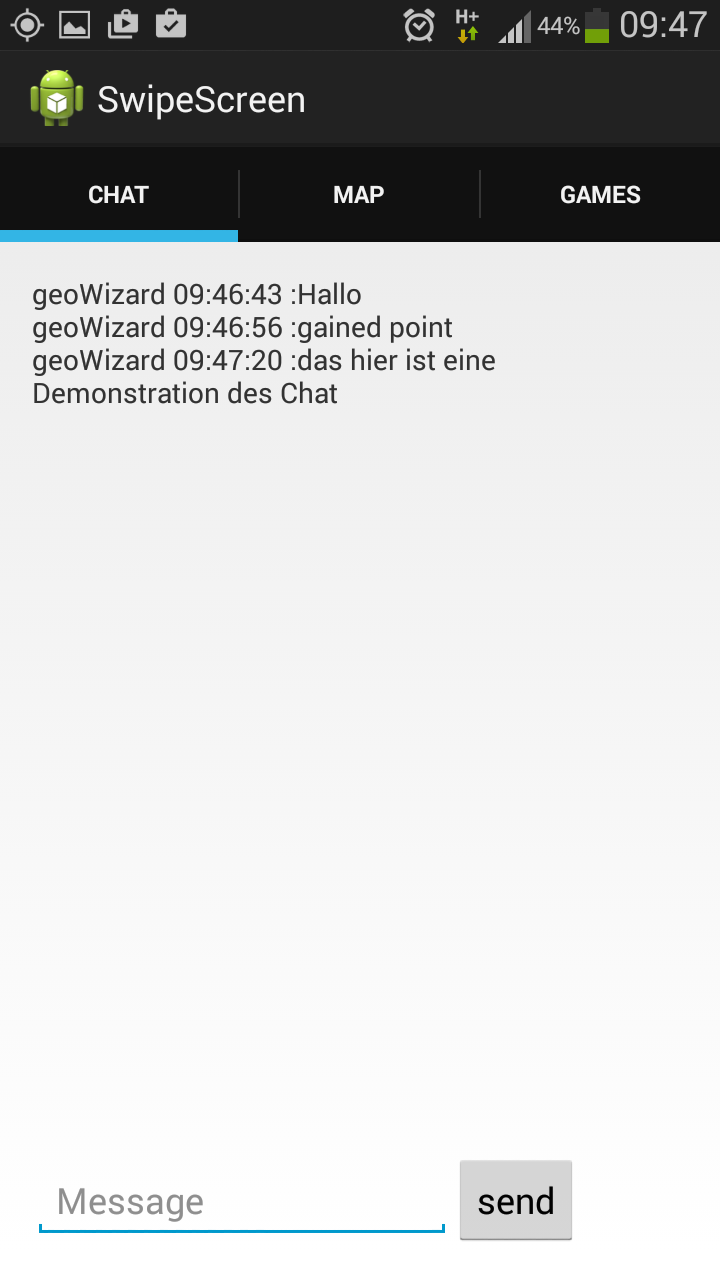
\includegraphics[width=0.48\textwidth]{4-Technische_Loesungen/4-5-GUI/Data/chat_screen.png}
     \caption{Chat Screen}
  \end{center}
\end{wrapfigure}

\subsubsection*{Chat-Screen}
In desem Fragment wird die m�glichkeit des Chattens zwischen mehreren Spielern umgesetzt. Die grafische Umsetzung des Chats wurde der von IRC (Instant Relay Chat) Clients nachempfunden und ist entsprechend simpel gel�st. Es wird der jeweilige Benutzername, Uhrzeit und die eigentliche Nachricht angezeigt. Die Eingabe der Chat-Nachricht erfolgt in einem Text-Eingabe-Feld. Die Anzeige der Chat-Nachrichten erfolgt in einem einfachen Textanzeige-Feld (TextView\footnote{{\url{http://developer.android.com/reference/android/widget/TextView.html}}}) was wiederum in einem scrollbaren Feld (SrcollView\footnote{\url{http://developer.android.com/reference/android/widget/ScrollView.html}}) liegt. Hierdurch ist es m�glich durch alle empfangenen Nachrichten "`durchzuscrollen"'. Wird eine Chat-Message (genaueres in Kapitel 4.4) empfangen, wird diese mittels Stringmanipulation an das Textfeld angeh�ngt. Hierbei ist zu beachten, dass die selbst verschickten Nachrichten erst an den Server gesendet werden und dann jeweils an die entsprechenden Nutzer. Somit kann es aufgrund von �bertragungsverz�gerungen dazu kommen, das die eigene Nachricht verz�gert angezeigt, jedoch ist die korrekte Reihenfolge der Nachrichten gewahrt.

\newpage

\begin{wrapfigure}{r}{0.5\textwidth}
  \begin{center}
    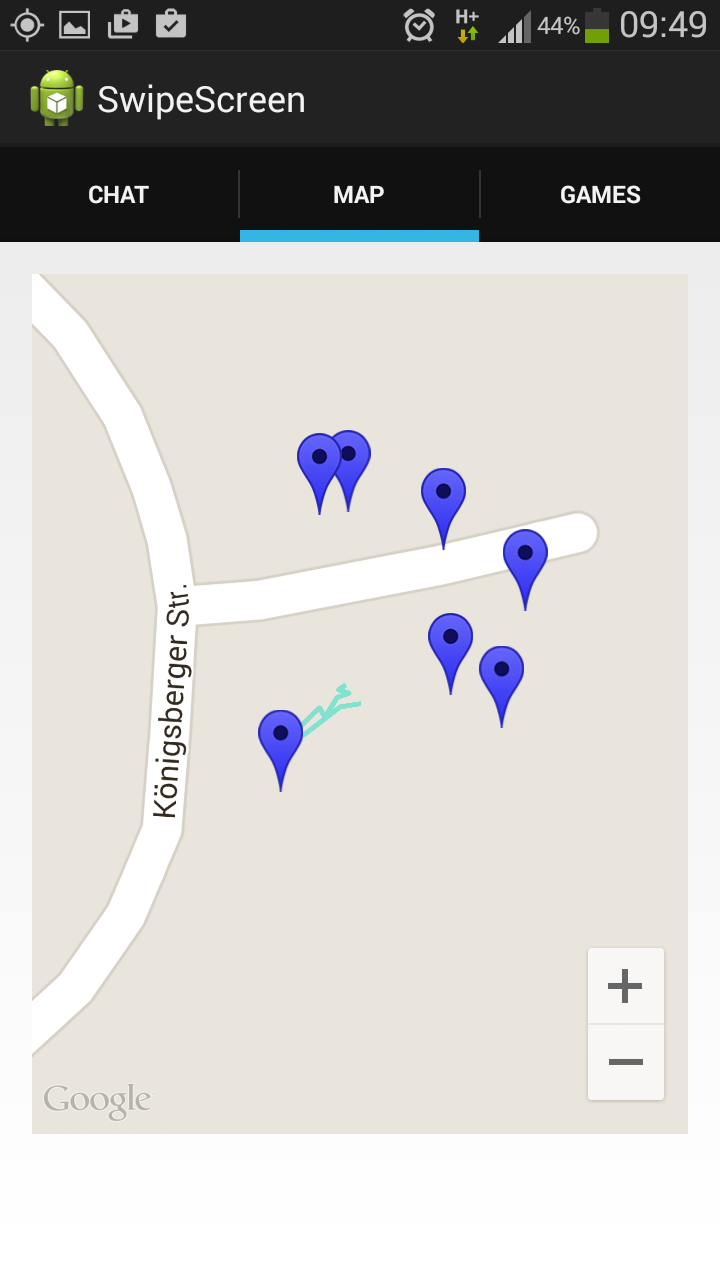
\includegraphics[width=0.48\textwidth]{4-Technische_Loesungen/4-5-GUI/Data/map_screen.png}
     \caption{Map Screen}
  \end{center}
\end{wrapfigure}

\subsubsection*{Map-Screen}
In diesem Fragment wird die Karte in einem weiterem Fragment angezeigt. Je nachdem welches Spiel gespielt wird zu zus�tzliche Widgets vorhanden, wie z.B. Interaktions Buttons, (Team-)Punkte anzeige usw.


\subsubsection*{Game-Screen}
In diesem Fragment werden momentan aktive Spiele angezeigt. Auch ist es m�glich neue Spiele zu erstellen. Die Anzeige der Liste der Spiele erfolgt in einer scrollf�higen Liste (ListView). Diese wird durch entsprechend angefordete Informationen �ber andere Spiele geupdatet. Diese Informationen werden durch Anfrage bei anderen Benutzer die sich eingeloggt haben �ber einen bestimmen Message-Typ abgerufen. Die Listen-Elemente sind interaktiv. Ein klick auf das entsprechende Spiel startet den beitritt. Um ein Spiel eines gewissen Typs zu Starten w�hlt man in einen Dropdown-Men� (bei Android Spinner) den entsprechenden Modus aus in klickt auf create. Man selbst betritt dieses Spiel und der Eintrag in der Spiele-Liste wird vorgenommen. 


\begin{figure}[r]  
    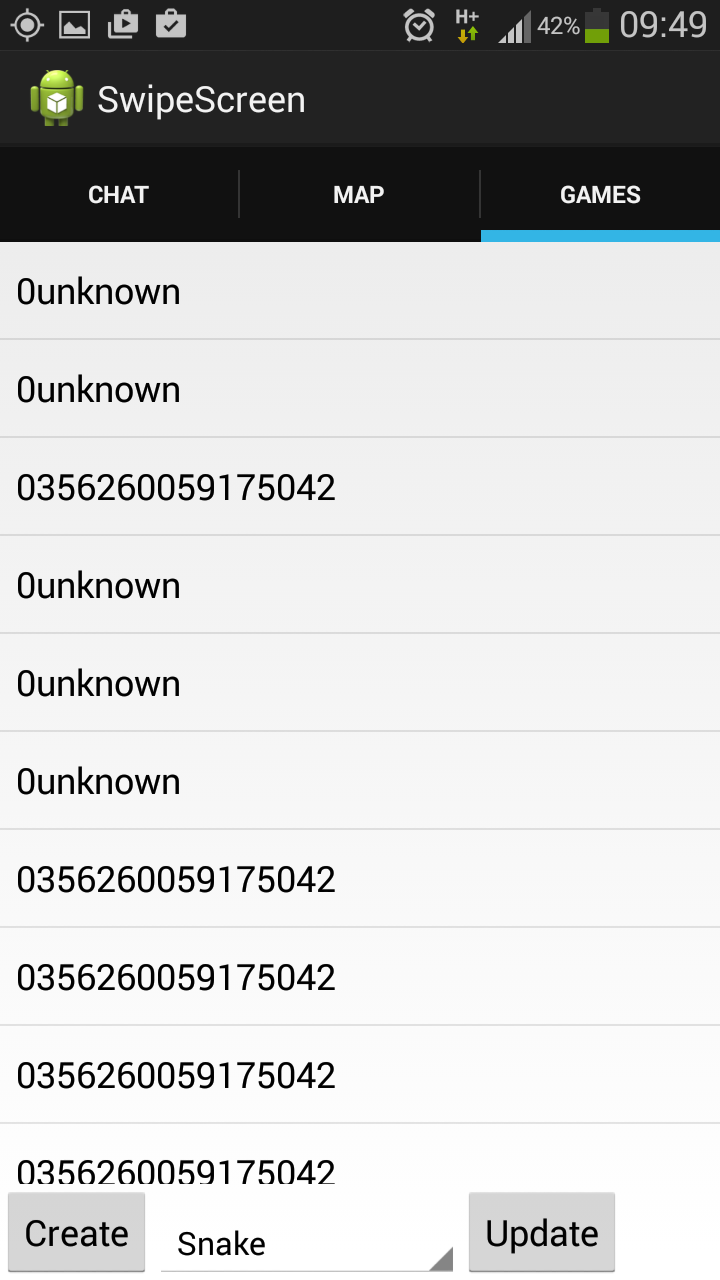
\includegraphics[width=0.48\textwidth]{4-Technische_Loesungen/4-5-GUI/Data/game_screen.png}
    \caption{Game Screen}
\end{figure}

\clearpage